\chapter{Foundations and Literature Review}
\label{chap:fundamentacao}
The tools and paradigms used on the work are: framework Apache Hadoop, MapReduce, context-awareness, as well as related works. They will be further explained in the following sections.

%-------------------------------------------------------------------

\section{Hadoop}
The Apache Hadoop framework was actually originated from another Apache \cite{Apache} project, the Apache Nutch \cite {Nutch}, which was an open source web search engine started on 2002. Unfortunately, Apache Nutch was facing problems due to its architecture, that was happening almost at the same time that Google published an article describing the architecture used on their distributed file system (GFS). The Nutch developers saw that a similar architecture to the GFS would solve Nutch's scalability problem.

In 2004 the Nutch developers began to implement the idea and the result was named Nutch Distributed Filesystem (NDFS). As the project advanced it began to take bigger and bigger proportions until 2006, when a new project was made because the advancements were bigger than Nutch's purpose. This new project was named Hadoop. The Hadoop framework has the purpose of facilitating distributed processing through the MapReduce paradigm.

\subsection{Apache Hadoop Architecture}
In a general view, it is possible to break Apache Hadoop in two parts. These parts are named Hadoop Distributed File System (HDFS) and Yet Another Resource Negotiator (YARN). Figure \ref{fig:ArqGeral} presents the aforementioned separation.

\begin{figure}[hbtn]
   \renewcommand{\figurename}{Figure}
   \centering
   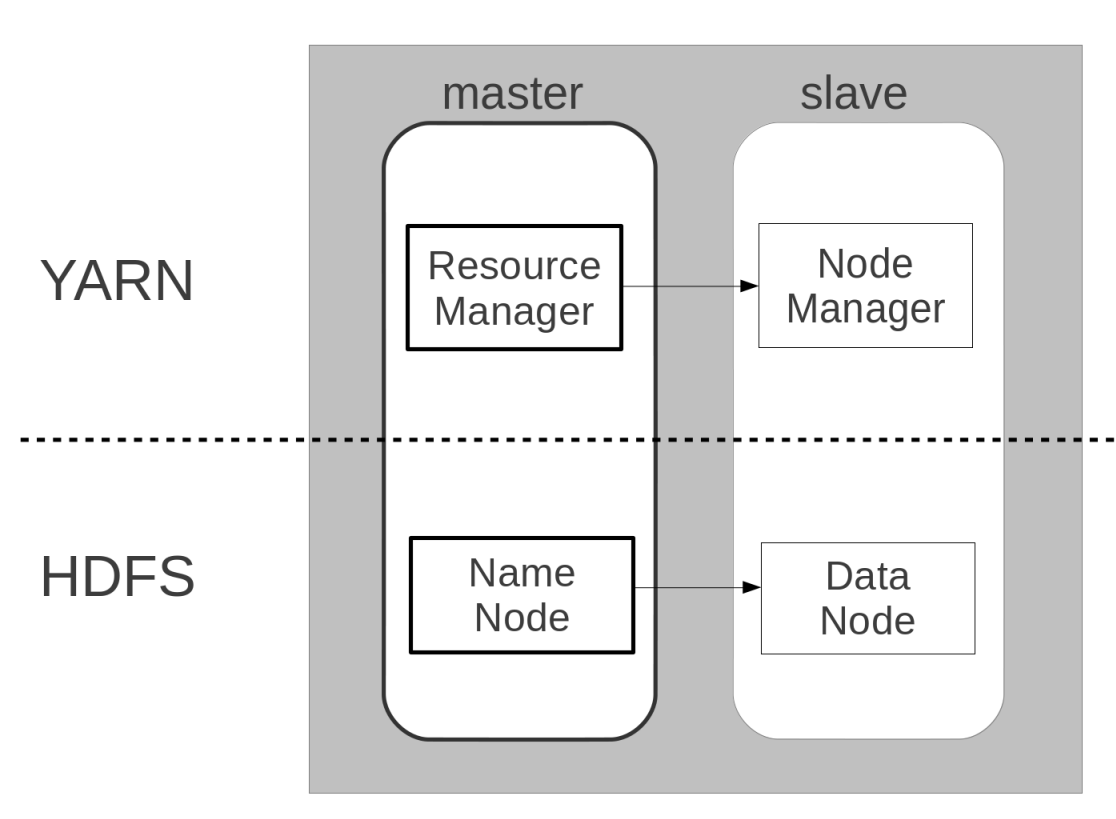
\includegraphics[width=9cm]{figuras/Figura08-HadoooArchGeral.png}
   \caption{General Apache Hadoop architecture}
   \label{fig:ArqGeral}
\end{figure}

HDFS is responsible for the data storage, which is required in order to execute jobs. It is the component which will replicate the data in order to provide fault tolerance, data distribution according to the requirements of each node, among other things.

YARN is the other half of Apache Hadoop, it is responsible for processing tasks from submitted jobs. It is through YARN components that the MapReduce tasks are executed, which consequently makes YARN the manager for all cluster resources.

\subsubsection{HDFS}
HDFS is in huge part responsible for Hadoop's good performance, because it has the task to not overloading the network with file transfers. Thanks to HDFS, the file access is always local, it means that every node will receive the file portion relative to its workload, thus preventing unnecessary replication other than for security and fault tolerance replication.

One problem of this approach is that Hadoop has a big latency, making its use inadvisable to critical or real time applications. The HDFS may be further divided in two services, NameNode and DataNode, responsible for the management of data in cluster level and local level, respectively. Figure \ref{fig:ArqHDFS} presents the basic HDFS architecture scheme.

\begin{figure}[hbtn]
   \renewcommand{\figurename}{Figure}
   \centering
   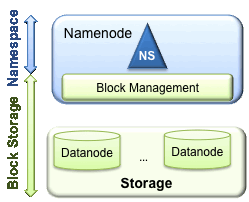
\includegraphics[width=8cm]{figuras/Figura07-HDFS.png}
   \caption{General HDFS architecture \cite{HDFS}}
   \label{fig:ArqHDFS}
\end{figure}

\subsubsection{YARN}
YARN is the portion of Apache Hadoop responsible for MapReduce execution, therefore the execution of management and processing tasks are controlled by YARN. In making the processing tasks totally independent from data storage tasks, the Apache Hadoop opens a lot of possibilities for it's utilization. Just like HDFS, YARN can be further divided into two services, ResourceManager and NodeManager, responsible for system resource management and local resource management, respectively. Figure \ref{fig:ArqYARN} presents the basic YARN's architecture scheme.

Although not shown on the figure, each service has many internal modules, for example the ResourceManager has the scheduler and the ApplicationsManager, which could still be further divided into sub-modules. The present work aims to present an improved solution for the scheduling and resource collection employed on Hadoop so it can adapt better to the environment.

\begin{figure}[hbtn]
   \renewcommand{\figurename}{Figure}
   \centering
   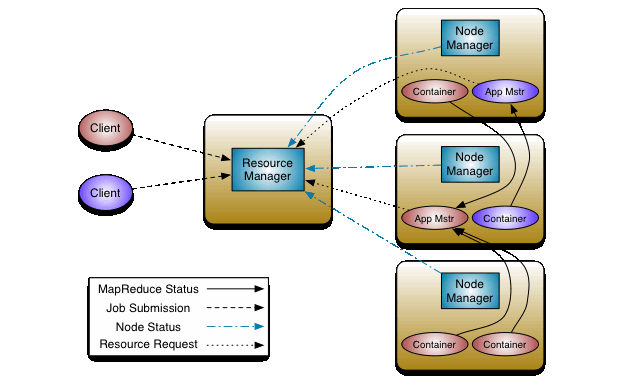
\includegraphics[width=12cm]{figuras/Figura06-YarnArch.png}
   \caption{General YARN architecture \cite{YARN}}
   \label{fig:ArqYARN}
\end{figure}

\subsection{Hadoop execution environment configuration}
\label{sec:envconfig}
A correctly configured Hadoop environment has a few pre-requisites besides having access between the nodes in a network. Every node must have in it's Hadoop installation many files, in XML format, containing the Virtual Machines' (VMs) configuration on that node.

The XML files are: core-site.xml, yarn-site.xml, mapred-site.xml, hdfs-site.xml. Each one of these files will contain one Hadoop service configuration. In case a parameter isn't set on these files, the VM will get the value from one of the *-default.xml files which contains the default Hadoop configuration. Although it may seem like an automated configuration, it is only a default value Hadoop will use in case no other value has been specified.

\subsection{MapReduce}
The MapReduce paradigm, already mentioned many times on the present work, breaks down the processing of tasks in two steps. These two steps are derived from functional language functions Map and Reduce which, just like their original implementations, work based on key and value tuples. The standard work-flow of a MapReduce application starts with the Map function receiving an input file and searching for application desired information, after this information is found it creates key and value tuples. 

Once the tuples are made the Map function sends them to Reduce function, where the keys will be processed and reduced to intelligible data. The Hadoop's greatest advantage is that, given a properly configured environment, the programmer can focus his attention and efforts on solving the tasks through MapReduce paradigm and not on making the tasks work properly distributed. Thus instead of having to worry about fault tolerance, scalability, and many other characteristics, the programmer will just focus on his algorithm.

%-------------------------------------------------------------------

\section{Context-awareness}
\label{sec:ctx}
Given the interactivity of today's systems, it is possible to note some context-aware applications already in use on most of them. For example, when a site is accessed through a mobile device it will automatically load the mobile version on the device in order to have optimized spacing and content designed for that kind of devices. Another example is when the browsers take into account geographical data from the user point of access and refine the search results towards that area. Also, it is possible to use an user navigation historic to predict which products and offers will arouse more interest on that person. 

All the above cases exemplified a situation where the application used some context in order to make a decision, making that application context-aware. But what really means to be a context-aware application? In order to answer this question there are two things that must be understood first, the definition of context and context-aware. 

Starting with the first, what would the so called context mean. This definition is fundamental in order to understand what is a context-aware system and context-aware itself \cite{Manuele}. Context can assume a lot of meanings depending on the situation, \cite{Dey} defines context as any information possible to be used in order to characterize an entity (person, place or object) considered relevant to the interaction between user and application.

Knowing what context is, it is possible to understand the context-aware definition made by \cite{Zakaria} in which he claims that context-aware is the ability of an application to detect and respond to changes in the execution environment. Which then can be complemented by the following definition made by \cite{Baldauf}, in which he defines a context-aware system as something capable of adapting it's operations to the actual context without explicit user intervention and therefore improve the usability and efficacy. 

Although there are many different methods to improve the MapReduce's performance through employment of context information, \cite{Manuele} suggests three possible ways to do so. These three methods are: automated node configuration on Hadoop installation/start-up, management of node removal and addition in real time and finally through scheduler task distribution according to the available resources and already executing tasks at any given time. The present work used a hybrid approach between the second and third suggestions, as it will collect the real node data and also impact on scheduling resource distribution.

%-------------------------------------------------------------------

\section{Hadoop Schedulers}
\label{sec:Hadoop Schedulers}
One of the Hadoop's main components is the scheduler. It is responsible for the resource and workload distribution among the environment. 

\subsection{Hadoop Internal Scheduler}
The standard Hadoop scheduler, was implemented aiming to support only batch job submission. It takes the first job received and executes it, making a queue for subsequent submissions. This scheduler supports five levels of priority, yet the choice for the next job to be executed will always take into account the submission time.

\subsection{Fair Scheduler}
Used for computing of small batch jobs that have the same input data size, using a two level scheduling in order to distribute the resources equally \cite{FairScheduler}. The superior level, usually allocates queues for each user, using a weighted fair algorithm. The second level allocates the resources inside each user queue, the scheduling in this level uses the same algorithm as Internal Scheduler.

\subsection{Capacity Scheduler}
This scheduler was implemented aiming the cases where the Hadoop environment is shared among various companies or has many distributed parts on places under multi-tenant responsibility. It focuses on guarantees that a minimum share will always be available for each company. The benefit comes from the fact that different organizations have processing peaks at different times, therefore the organization using more capacity, will use the idle capacity of the other organizations. This is the most complete scheduler provided by Hadoop. It is able to track the resources registered within the RM, although not consistent with the reality, and monitor which resources are free and which are being used.

%-------------------------------------------------------------------

\section{Related work}
Beyond the schedulers patched together with Hadoop, there are other implementations that sought to solve a specific necessity that the standard schedulers do not offer support. A bibliographic research was made aiming to analyze the works already published involving Hadoop and having as purpose adapting or changing the scheduling. Besides, it was sought to identify which techniques were the most used and which were the most common objectives of the developed work. Following, there is a list of the related works containing a brief abstract of their proposals, used context and expected objective with the interventions.

\begin{itemize}
	\item CASH (Context Aware Scheduler for Hadoop) \cite{CASH}, this work had the objective of improving the cluster overall performance. Assuming the hypothesis that a huge part of the jobs are periodic and executed at roughly the same time, while also having similar CPU, network and disk usage characteristics. The work still takes into account that with time the nodes tend to become heterogeneous. With the intention to solve this situation, a scheduler that classifies both jobs and nodes with respect to its CPU or I/O potential was implemented, it can then distribute the jobs for machines with a more appropriated configuration regarding the job's nature.

	\item LATE (Longest Approximation Time to End) \cite{LATE}, following what the name suggests, in this work context information is regarded to a job's estimated time to end, this time is based on a heuristic that makes the connection between elapsed time and the score. Score is a value that represents how much of the job has already been processed. This information is used to generate a threshold which will determine when a task is slow enough to start a new speculative copy on another possibly faster machine. The objective of this work was to reduce the response time in large clusters executing many jobs of short duration.

	\item A Dynamic MapReduce Scheduler for Heterogeneous Workloads \cite{DMRSHW}, the authors of this work used the technique of classifying the jobs and machines according to the I/O and CPU potential. Just like CASH the main objective is the improvement of cluster performance. One of the differences however, is that this implementation uses a three queue scheduler.

	\item SAMR (A Self-adaptative MapReduce) \cite{SAMR}, this implementation follow the same idea from LATE, where the context information refers to the job progress calculation and is used to identify if it is necessary to launch a speculative task. However, this solution changes a bit the calculation of progress by inserting information about the job's execution environment, the algorithm takes into account historical informations contained in each node and uses it to adjust weight of each processing step.

	\item COSHH (A Classification and Optimization based Scheduler for Heterogeneous Hadoop Systems) \cite{COSHH}, a wider proposal if compared to the rest of the solutions, this one takes into account informations not specified about the system. It's performance gain is achieved through classification of jobs in classes, then it searches the whole cluster for machines that match the same class as the job. This search is made by an algorithm that reduces the search sample size, thus improving search response and performance. The objective of this solution is the improvement of medium job completion time, besides offering a good performance when using the minimum share and providing a fair distribution of resources.

	\item Quincy \cite{Quincy}, this solution was not proposed solely for Hadoop environments, but still applicable to it. Possessing the objective of improving general cluster performance, uses the distribution of resources as context information and modifies the traditional way of treatment to these. In using a more dynamic approach, the solution maps the resources in a capacity-demand graph and calculates the optimum scheduling from a global cost function.

	\item Improving MapReduce Performance through Data Placement in heterogeneous Hadoop Clusters \cite{IMRPDPHHC}, this 	solution aims to provide better performance on jobs through better data placement, using mainly the data locality as decision making information. The performance gain is achieved by the data re-balancing in nodes, leaving faster nodes with more data. This lowers the cost of speculative tasks and also of data transfers through the network.
\end{itemize}

After studying the related works, it is possible to note that many of them have the reduction of response time or improvement of overall performance as objective, which are slightly different from the present work that aims firstly for a better Hadoop adaptation in a heterogeneous environment, which will consequently provide a better performance.
Regarding the context, there were many contexts used although, it is possible to identify recurrent contexts such as: job classification according I/O and CPU potential, job progress evaluation in order to launch or not speculative tasks.